

% case 2 result

\section{Case overview}



\section{Quantitative analysis}

\subsection{Descriptive statistics}

\subsubsection{Demographics}

Of the 25 participants invited to take part in Case Two, all agreed to participate (100\% response rate). Seven participants were female, the rest were male. The age of participants ranged from 26 to 68 years (average age = 44 years, median age = 41 years). Relevant work experience ranged from 1 to 40 years (average experience = 14.9 years, median experience = 12 years). Current job tenure ranged from 1 to 40 years (average tenure = 13.4 years, median tenure = 10 years). Box-plots showing the distribution of age, work experience and tenure of participants in each case study are presented in Figure \ref{fig:ageexperience}.\medskip

The participants in Case Two are based in three countries. Figure \ref{fig:sphdistancecase2} depicts the spherical distance between every participant in the collaboration (calculated using their work-place postcodes as a geographic reference). Most of the participants are either co-located or within reasonable driving distance of each other. However, four individuals (nodes 8, 10, 13, 14) are located in a different part of the same country, three individuals (nodes 9, 18, 22) are from a neighbouring country, while three nodes (nodes 23, 24, 25) are based on another continent.\medskip

Figure \ref{fig:edlevelrose} shows how education levels differ in each case study. Participants in this case study have education levels ranging from secondary level to doctoral level. Most participants have a tertiary qualification in agriculture. Other participants have educational backgrounds in natural and physical sciences, engineering, mixed field programmes, management, or education (Figure \ref{fig:edfieldrose}). 

\subsubsection{Basic network statistics}

Descriptive statistics for the explicit and tacit knowledge provider networks and idea contributor network are presented in Table \ref{ds_c2}. All three networks are based on a common set of nodes (25 in total). The networks are reasonably dense with a number of reciprocated ties, indicating there is a high level of social interaction in Case 2. Of the three networks, the idea contributor network is the most dense, followed by the tacit knowledge provider network. This suggests the innovation challenge in this instance is complex, demanding greater levels of tacit knowledge exchange and creative interaction.\medskip

\begin{table}[]
	\small
	\centering
	\caption{Descriptive network statistics - Case 2}
	\label{ds_c2}
	\begin{tabular}{@{}lcccccc@{}}
		\toprule
		& \multicolumn{1}{l}{} & \multicolumn{1}{l}{} & \multicolumn{1}{l}{} & \multicolumn{3}{c}{Dyad Census}	\\ \cline{5-7}
		Network						& Nodes			& Arcs			& Density	& Mutual		& Asymmetric	& Null		\\ \midrule
		Explicit Knowledge Provider & 25			& 105			& 0.18		& 13			& 79			& 208		\\
		Tacit Knowledge Provider    & 25			& 133			& 0.22		& 22			& 89			& 100		\\
		Idea Contributor            & 25			& 141			& 0.24		& 31			& 79			& 190		\\ \bottomrule
	\end{tabular}
\end{table}

Figure \ref{fig:thesisnetworkscase2} depicts network diagrams for all three networks. Arrows indicate the direction of knowledge and idea flows. Nodes are sized according to Burt's constraint measure (the larger the node diameter, the greater the node's access to knowledge or ideas) and coloured according to employer affiliation. Judging by the size of nodes, individuals in all three networks are for the most part not very constrained in terms of accessing network resources. One individual, who stands out as having the greatest access to explicit knowledge, does not enjoy the same level of access to tacit knowledge and ideas (node 18). This person is a senior executive who keeps tabs on what is going on in the collaboration but does not get too involved in actual problem-solving or development activities.\medskip 

\begin{landscape}
	\begin{figure}
		\centering
		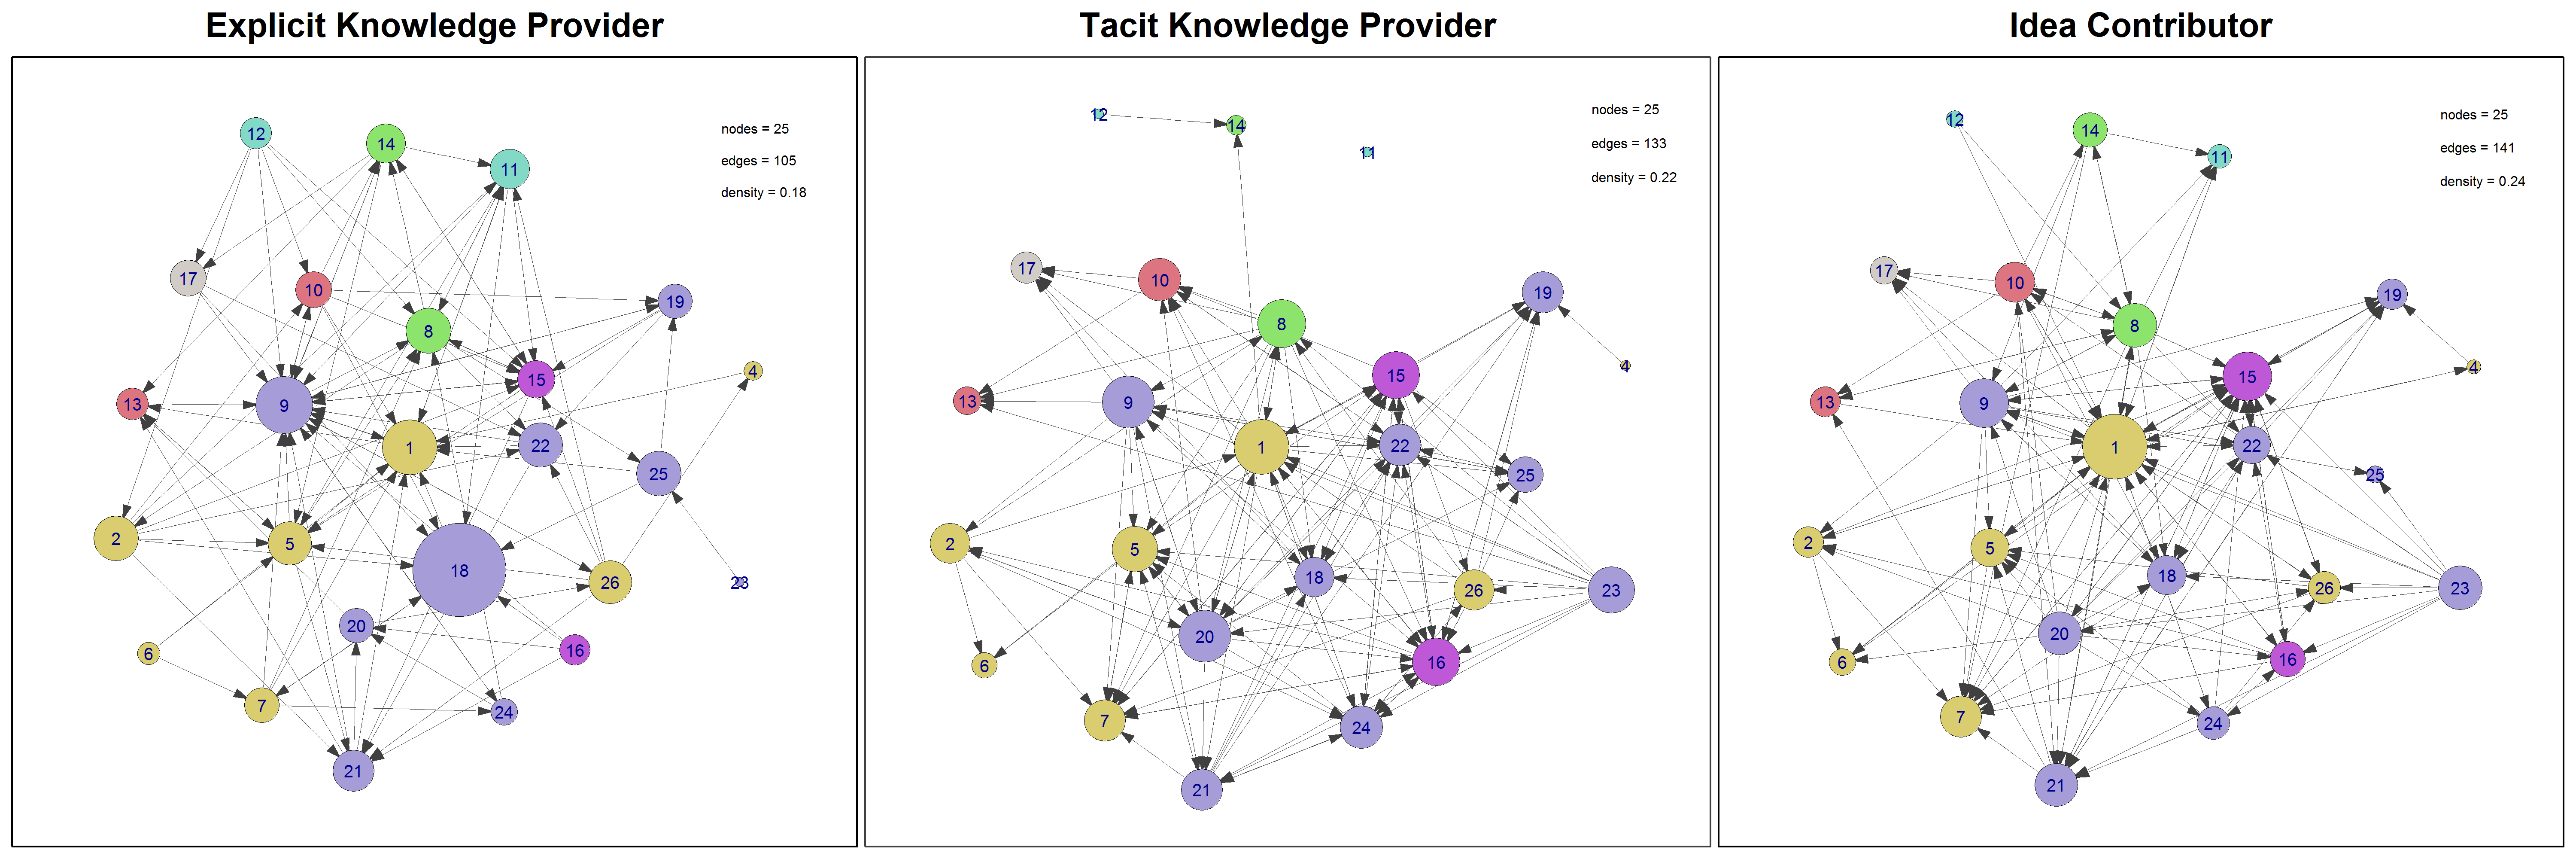
\includegraphics[width=1.0\linewidth]{Images/thesis_networks_case2}
		\caption{Network diagrams - Case 2}
		\label{fig:thesisnetworkscase3}
	\end{figure}
\end{landscape}



\begin{figure}
	\centering
	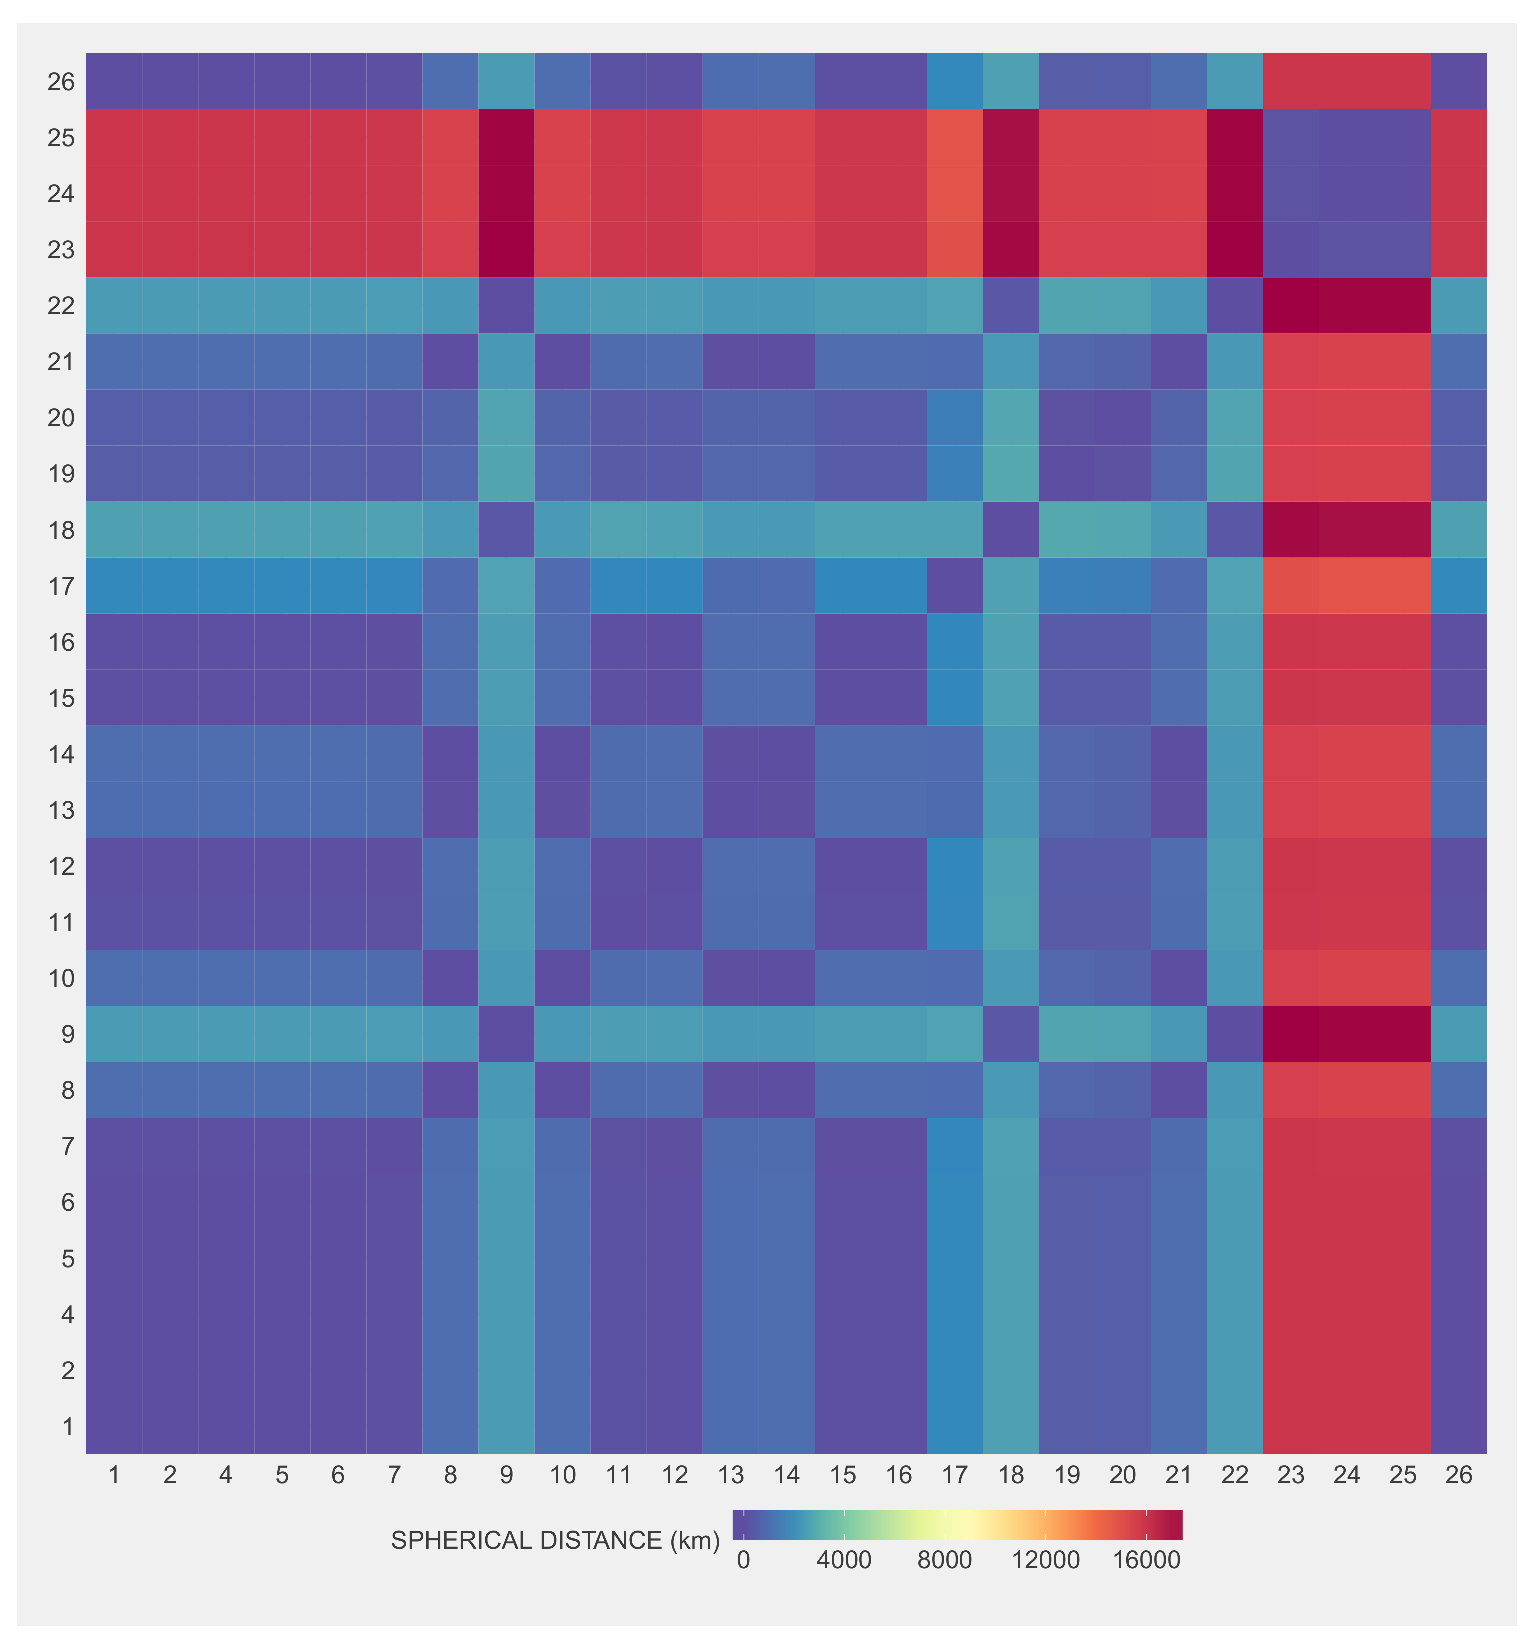
\includegraphics[width=0.7\linewidth]{Images/sph_distance_case2}
	\caption{Distance between nodes - Case 2}
	\label{fig:sphdistancecase2}
\end{figure}

\subsubsection{Two-path brokerage statistics}

A breakdown of different broker roles in the explicit and tacit knowledge provider networks and idea contributor network according to employer affiliation is presented in Figure \ref{fig:gfbrokeragecase2}. Liaison is the dominant form of brokerage in the explicit knowledge provider network (as was observed in Case 1). This implies individuals have a tendency to broker explicit knowledge between different organisations. The tacit knowledge provider network has a wide spread of different broker roles. This indicates tacit knowledge features strongly in a broad range of interactions between partner organisations. The relatively high levels of brokerage in the idea contributor network suggests there is much creative interaction with many ideas flowing out organisations into others via third-parties. Liaison is dominant in all three networks, indicating there is a good level of collaboration amongst partner organisations. \medskip 

\begin{figure}
	\centering
	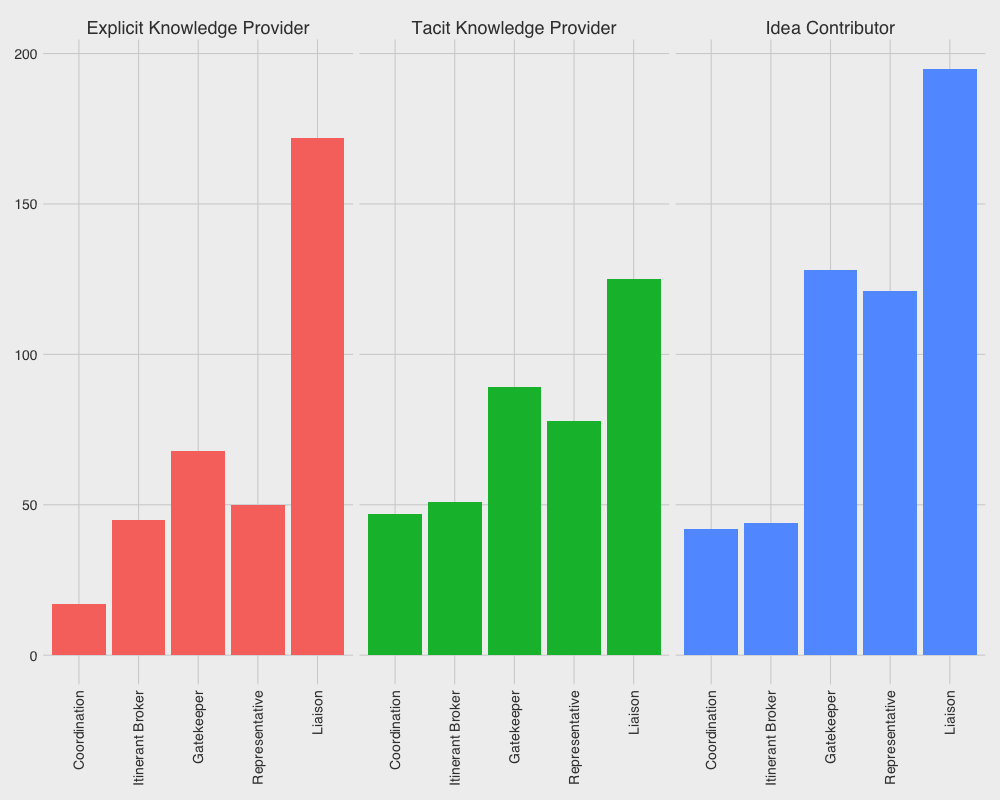
\includegraphics[width=0.7\linewidth]{Images/gf_brokerage_case2}
	\caption{Gould-Fernandez brokerage roles - Case 2}
	\label{fig:gfbrokeragecase2}
\end{figure}

\subsection{Exponential random graph modelling}

\subsubsection{Autonomous motivation as a predictor of knowledge sharing}

Both the explicit and tacit knowledge provider networks were modelled to determine if autonomous motivation predicts knowledge sharing behaviour in Case 2. Table \ref{c2_q1} contains the parameter estimates with standard errors in brackets for the explicit knowledge provider and tacit knowledge provider networks (Models F and G respectively). The estimation procedure successfully converged for all the modelled parameters. Goodness of fit statistics show both models fit the data very well (the statistics were less than 1 in absolute value for almost all the features not explicitly modelled). As before, results are broken down according to purely structural effects, actor-relation effects, and network covariate effects. \medskip

Looking at the results for purely structural effects, there is a significant and positive effect for popularity spread in the explicit knowledge provider network, indicating some actors are receiving significantly more explicit knowledge than others. Results for the tacit knowledge provider network show a significant and positive effect for path closure and a significant and negative effect for multiple connectivity. Path closure indicates a tendency to close structural holes whereas multiple connectivity refers to a tendency for brokerage. The combination of a positive path closure and negative multiple connectivity effect implies a collaboration mechanism is driving tacit knowledge sharing.\medskip

With respect to actor-relation effects, there is a strong and positive sender and receiver effect for autonomous motivation with respect to tacit knowledge sharing (Model G). There is a significant and positive sender effect for work experience in Model F indicating more experienced individuals are more likely to share explicit knowledge. The significant and positive effect for identification with the collaboration in Model F suggests individuals who identify more strongly with the collaboration are also more likely to share explicit knowledge. The significant and positive effect for employer match in Model G indicates a tendency for people are more likely to share tacit knowledge with fellow employees. Interestingly, the significant and negative sender effect for education level in Model G implies more educated people are less likely to share tacit knowledge with others in the collaboration. Regarding network covariate effects, there is a significant and positive effect for hierarchy in Model F, indicating individuals are more likely to share explicit knowledge with those they report to in the collaboration.\medskip

What the modelling tells us about the extent to which autonomous motivation predicts knowledge sharing behaviour is that autonomous motivation has no significant effect on explicit knowledge sharing but does have a significant effect on tacit knowledge sharing. The modelling also suggests a collaboration mechanism lies at the heart of tacit knowledge sharing.


\begin{table}[]
	\centering
	\caption{Autonomous motivation as an antecedent for knowledge sharing - Case 2}
	\label{c2_q1}
	\begin{threeparttable}
		\begin{tabular}{@{}lrlrl@{}}
			\toprule
			& \multicolumn{4}{@{}c@{}}{Estimate (SE)}   \\ \cline{2-5} 
			& \multicolumn{2}{@{}c@{}}{\begin{tabular}[c]{@{}c@{}}Explicit\\ Knowledge\end{tabular}} & \multicolumn{2}{@{}c@{}}{\begin{tabular}[c]{@{}c@{}}Tacit\\ Knowledge\end{tabular}} \\ \midrule
			\textbf{Purely structural effects (endogenous)} &			&          	&         	&         	\\
			Arc (edge)         								& -4.130  	& (1.916)* 	& -2.296  	& (1.470) 	\\
			Reciprocity (mutuality)                         & -0.237  	& (0.910)   & -0.360  	& (0.625) 	\\
			TwoPath (simple connectivity)                   & 0.065   	& (0.044)  	& -0.024  	& (0.042) 	\\
			AinS (popularity spread)                        & 0.825   	& (0.392)* 	& 0.324 	& (0.392) 	\\
			AoutS (activity spread)                         & -0.972  	& (0.742)  	& 0.524 	& (0.412) 	\\
			AT-T (path closure)                             & 0.104   	& (0.192)  	& 0.743 	& (0.248)*	\\
			AT-C (cyclic closure)                           & 0.145   	& (0.146)  	& 0.000 	& (0.127) 	\\
			A2P-T (multiple connectivity)                   & -0.099  	& (0.080)   & -0.203  	& (0.063)*	\\
															&         	&          	&       	&         	\\
			\textbf{Actor-relation effects (exogenous)}     &         	&          	&       	&         	\\
			age (difference) 								& -0.009  	& (0.012)  	& 0.012 	& (0.012) 	\\
			work.experience (sender)                        & 0.036   	& (0.016)* 	& -0.002  	& (0.008) 	\\
			work.experience (receiver)                      & -0.002  	& (0.013)  	& -0.010  	& (0.010)  	\\
			education.level (sender)                        & 0.191   	& (0.105)  	& -0.160  	& (0.067)*  \\
			education.level (receiver)                      & -0.007  	& (0.069)  	& -0.063  	& (0.068) 	\\
			personality.openness (sender)                   & -0.592  	& (1.165)  	& 0.469 	& (0.639) 	\\
			personality.openness (receiver)                 & -0.525  	& (0.808)  	& 0.492 	& (0.661) 	\\
			self.efficacy (sender)                          & 1.021   	& (1.441)  	& -1.534  	& (0.866) 	\\
			self.efficacy (receiver)                        & 0.420   	& (1.114)  	& -1.884  	& (0.959) 	\\
			identification.collab (product)                 & 2.094   	& (0.968)* 	& -0.590  	& (0.632) 	\\
			autonomous.motivation (sender)                  & -1.549  	& (1.147)  	& 1.650 	& (0.707)*  \\
			autonomous.motivation (receiver)                & 0.874   	& (0.825)  	& 1.590 	& (0.768)*  \\
			broad.education.field (match)                   & -0.061  	& (0.227)  	& 0.082 	& (0.212) 	\\
			employer (match) 								& 0.299   	& (0.396)  	& 0.727 	& (0.325)*  \\
			employer (mismatch reciprocity)                 & 0.724   	& (0.990)   & 0.902 	& (0.653) 	\\
															&         	&          	&       	&         	\\
			\textbf{Network covariate effects (exogenous)}  &         	&          	&       	&         	\\
			report.to.net (hierarchy)                       & 1.291   	& (0.391)*	& -0.516  	& (0.433) 	\\
			log.spherical.distance.net (spatial proximity)  & 0.023   	& (0.048)  	& -0.043  	& (0.045) 	\\ \bottomrule
		\end{tabular}
		\begin{tablenotes}
			\small
			\item [*] Significant effect.
		\end{tablenotes}
	\end{threeparttable}
\end{table}

\subsubsection{Brokerage versus level of tacit knowledge exchange}

Work in progress.

\subsubsection{Role of tacit knowledge in creative interaction}

Model H assesses the influence of tacit knowledge on idea contribution in context of creative interaction. Table \ref{c2_q3} contains the parameter estimates with standard errors in brackets for Model H. The estimation procedure successfully converged for all the modelled parameters. Goodness of fit statistics were under 2 in absolute value for features not explicitly modelled, indicating Model H fits the data well. Results are again broken down according to purely structural effects, actor-relation effects, and network covariate effects.\medskip 

Examining the purely structural effects, there is a significant and positive effect for path closure and multiple connectivity in Model H. This suggests there is good socialisation of ideas but that sharing of ideas involves significant brokerage. The significant and negative effect for cyclic closure indicates individuals engage in creative interaction selectively.\medskip

Regarding actor-relation effects, there is a significant and positive sender effect in Model H for autonomous motivation. Individuals with higher levels of autonomous motivation are more likely to contribute ideas. Surprisingly, there is a significant and negative sender effect for self-efficacy. Individuals who feel competent at their job, enjoy a fair amount of autonomy, and who also consider themselves to be creative, are less likely to contribute ideas!\medskip

In terms of network effects, there is significant and positive dyadic covariate effect for both the explicit and tacit knowledge provider networks. In other words, idea contribution ties are more likely to emerge in the presence of existing knowledge sharing ties. As with Case 1, the effect is stronger for the tacit knowledge provider network implying there is a stronger tendency for creative interaction to happen between people who exchange tacit knowledge. There is also a significant and negative effect for spatial proximity, indicating individuals are more likely to contribute ideas to others in close proximity. \medskip  

\begin{table}[]
	\centering
	\caption{Tacit knowledge sharing as an antecedent to creative interaction - Case 2}
	\label{c2_q3}
	\begin{threeparttable}
	\begin{tabular}{@{}lrl@{}}
		\toprule
		& \multicolumn{2}{@{}c@{}}{Estimate (SE)} \\ \midrule
		\textbf{Purely structural effects (endogenous)}      &                &                  \\
		Arc (edge)                                           & -5.330         & (2.505)*         \\
		Reciprocity (mutuality)                              & -0.079         & (0.682)          \\
		TwoPath (simple connectivity)                        & -0.052         & (0.081)          \\
		AinS (popularity spread)                             & 0.780          & (0.639)          \\
		AoutS (activity spread)                              & 0.348          & (0.631)          \\
		AT-T (path closure)                                  & 0.701          & (0.301)*         \\
		AT-C (cyclic closure)                                & -0.351         & (0.144)*         \\
		A2P-T (multiple connectivity)                        & 0.257          & (0.113)*         \\
		&                &                  \\
		\textbf{Actor-relation effects (exogenous)}          &                &                  \\
		age (difference)                                     & 0.003          & (0.016)          \\
		work.experience (sender)                             & -0.028         & (0.016)          \\
		work.experience (receiver)                           & 0.019          & (0.014)          \\
		education.level (sender)                             & -0.124         & (0.111)          \\
		education.level (receiver)                           & -0.013         & (0.093)          \\
		personality.openness (sender)                        & 2.031          & (1.238)          \\
		personality.openness (receiver)                      & 0.145          & (1.09)           \\
		self.efficacy (sender)                               & -4.536         & (1.757)*         \\
		self.efficacy (receiver)                             & 1.236          & (1.454)          \\
		identification.collab (product)                      & -0.948         & (1.083)          \\
		autonomous.motivation (sender)                       & 2.485          & (1.137)*         \\
		autonomous.motivation (receiver)                     & 0.718          & (0.994)          \\
		broad.education.field (match)                        & 0.084          & (0.303)          \\
		employer (match)                                     & 0.341          & (0.449)          \\
		employer (mismatch reciprocity)                      & 0.808          & (0.75)           \\
		&                &                  \\
		\textbf{Network covariate effects (exogenous)}       &                &                  \\
		tacit.knowledge.net (tacit knowledge provider)       & 3.730          & (0.406)*         \\
		explicit.knowledge.net (explicit knowledge provider) & 1.987          & (0.405)*         \\
		report.to.net (hierarchy)                            & 0.911          & (0.497)          \\
		log.spherical.distance.net (spatial proximity)       & -0.268         & (0.062)*         \\ \bottomrule
		\end{tabular}
		\begin{tablenotes}
			\small
			\item [*] Significant effect.
		\end{tablenotes}
	\end{threeparttable}
\end{table}


\section{Qualitative analysis}

\begin{landscape}
	\begin{table}[]
		\centering
		\caption{Case 2 interview participants}
		\label{c2_interviews}
		\begin{threeparttable}
			\begin{tabular}{@{}cccccccccccc@{}}
				\toprule
				Node & Employer & \begin{tabular}[c]{@{}c@{}}Interview \\ Date\end{tabular} & Age & \begin{tabular}[c]{@{}c@{}}Relevant\\ Work \\ Experience\end{tabular} & \begin{tabular}[c]{@{}c@{}}Current \\ Job \\ Tenure\end{tabular} & \begin{tabular}[c]{@{}c@{}}Education\\ Level\end{tabular} & \begin{tabular}[c]{@{}c@{}}Broad\\ Education\\ Field\end{tabular} & \begin{tabular}[c]{@{}c@{}}In-degree\\ Centrality\end{tabular} & \begin{tabular}[c]{@{}c@{}}Out-degree\\ Centrality\end{tabular} & \begin{tabular}[c]{@{}c@{}}Eigenvector\\ Centrality\end{tabular} & \begin{tabular}[c]{@{}c@{}}Burt's\\ Constraint\\ Measure\end{tabular} \\ \midrule
				1        & 1   &  25/02/16     	& 28  & 7      & 7   	& 6      & 5   & 19   	& 20  & 0.95   & 0.16    \\
				8        & 2   &  17/03/16     	& 41  & 14     & 10  	& 8      & 5   & 12   	& 16  & 0.73   & 0.18    \\
				9        & 3   &  14/03/16     	& 46  & 18     & 8  	& 6      & 5   & 21  	& 19  & 1.00   & 0.17    \\
				10       & 4   &  18/03/16     	& 32  & 10     & 2  	& 8      & 5   & 9  	& 9   & 0.50   & 0.20    \\
				11       & 5   &  29/02/16     	& 58  & 25     & 8  	& 6      & 1   & 5  	& 6   & 0.34   & 0.24    \\
				15       & 6   &  03/11/16     	  	& 50  & 25     & 19  	& 4      & 3   & 18   	& 16  & 0.89   & 0.18    \\
				18       & 3   &  16/02/16     	& 68  & 5      & 35  	& 5      & 8   & 21   	& 5   & 0.59   & 0.14    \\
				23       & 3   &  11/03/16     	& 44  & 20     & 25  	& 3      & 3   & 0  	& 15  & 0.44   & 0.20    \\ \bottomrule
			\end{tabular}
			 \begin{tablenotes}
			 	\small
			 	\item Notes:
			 	\item 1. Numbers in the education level/broad education field columns are the same as those used in the Australian Standard Classification for Education.
			 	\item 2. Statistics for the undifferentiated knowledge provider network.
			 	\item 3. In-degree centrality refers to the number of incoming knowledge ties. Out-degree centrality refers to the number of outgoing knowledge ties.
			 	\item 4. Eigenvector centrality refers to the relative importance of a node (connectivity with other high degree-centrality nodes) on a scale of 0 to 1.
			 	\item 5. Burt's constraint measure refers to access to network resources on a scale of 0 to 1. Lower values mean greater access to network resources.
			 \end{tablenotes}
		\end{threeparttable}
	\end{table}
\end{landscape}
 
